%!TEX root = ./thesis.tex

\chapter{State of the art}
\label{cha:soa}

This chapter gives an theoretical overview of different topics covered in this for low precision arithmetic over \gls{fpga}. At first, \glspl{spn} are described. Then, we explain how floaint point and posit representation works and how they are used in this work.

A \gls{spn} is a deep network architecture for probabilistic inference. This Chapter explains what is the general architecture of a \gls{spn} and what are the different properties that it can have and how it will be used in this work.

Low precision arithmetic regroup different binary number encoding sheme to represent floating point numbers with a low number of bits. Two representations are studied: Floating point and posit.


% ==============================================================================
\section{Sum product networks}
% ==============================================================================

\begin{definition}{\Gls{spn}}
In \cite{spns}, a \gls{spn} is defined as a rooted acyclic graph with variables as leaves, sum and product as internal nodes, and weighted edges.
\end{definition}

\Glspl{spn} are a new deep network architecture that allow to perform graphical probabilistic inference. This architecture is differentiated to others by the fact that the function it represents is tractable. That is: the output of the network can be analysed given the inputs.

As an example, two graphical representations from \cite{spns} are shown in Figure \ref{fig:spn_example}. The leaves of this network are the indicators $X_i$ and $\bar{X_i}$. A \gls{spn} represent the probability $P(X_0, \bar{X_0}, ...,  X_N, \bar{X_N})$. If the input of the \gls{spn} is an image, the indicators whould be the pixel values (1 for black and 0 for white).

In order to compute a specific set of probability with the evidence that $X_i=0$, the input of the \gls{spn} $X_i$ must be set to $0$ and the indicator $\bar{X_i}$ must be set to $1$. In order to compute a specific set of probability and marginalize over the variable $X_i$, the indicators $X_i$ and $\bar{X_i}$ must both be set to $1$. In any case, the values of the indicator $X_i$ and $\bar{X_i}$ will never both be $0$ at the same time.

\begin{figure}[!ht]
\begin{mdframed}
	\includestandalone[width=0.43\linewidth]{../Images/spn_example1}
	\includestandalone[width=0.56\linewidth]{../Images/spn_example2}
	\caption{Examples of \glspl{spn} from \cite{spns}}
	\label{fig:spn_example}
\end{mdframed}
\end{figure}

% -----------------------------------------------------------------------------
\subsection{Properties}
% -----------------------------------------------------------------------------

Two properties are interesting for \glspl{spn}: it can be complete and consistent. If an \gls{spn} is complete and consistent, it represent a partition function and can be used to compute all the marginals of this partition function.

\begin{definition}{Complete}
A \gls{spn} is complete iff all children of the same sum node have the same scope. A counter example is shown in Figure \ref{fig:incomplete}.
\end{definition}

\begin{definition}{Consistent}
A \gls{spn} is consistent iff no variable appears negated in one child of a product node and non-negated in another. A counter example is shown in Figure \ref{fig:inconsistent}.
\end{definition}

\begin{figure}[!ht]
\begin{mdframed}
	\centering
	\subfloat[incomplete]{\includestandalone{../Images/incomplete} \label{fig:incomplete}}
	\subfloat[inconsistent]{\includestandalone{../Images/inconsistent} \label{fig:inconsistent}}
\end{mdframed}
\end{figure}

% -----------------------------------------------------------------------------
\subsection{Applications}
% -----------------------------------------------------------------------------

\Glspl{spn} have a wide range of applications. A GitHub repository is dedicated to list and all ressources about \glspl{spn} and related work \cite{awesome_spn}. A wide range of machine learning problems can be solved with \gls{spn} such as regression or classification. As an example, there is \cite{spn_classification} which classify images using \glspl{spn} for autonomous flight.

% -----------------------------------------------------------------------------
\subsection{PSDDs}
% -----------------------------------------------------------------------------

\Glspl{psdd} are a specific kind of \gls{spn}. It was first reported in \cite{psdd_0}. \Glspl{psdd} are composed of three kind of nodes described in Figure \ref{fig:psdd2spn}: Literal nodes (leafs), true nodes and decomposition nodes.

This work uses pre-trained \gls{psdd} networks to generate \glspl{spn} in \gls{hdl}. The networks used in work are trained using a method described in \cite{psdd_1}.

\begin{figure}[!ht]
\begin{mdframed}
  \centering
  \subfloat[Literal node]{\includestandalone[scale=0.9]{../Images/literal_node}} \hspace{00.5cm}
  \subfloat[True node]{\includestandalone[scale=0.75]{../Images/true_node}} \hspace{0.5cm}
  \subfloat[Decomposition node]{\includestandalone[scale=0.75]{../Images/decomp_node}}
  \caption{Decomposition of PSDD file into simple arithmetic expression for \gls{spn} format.}
  \label{fig:psdd2spn}
\end{mdframed}
\end{figure}


% ==============================================================================
\section{Low precision arithmetic}
% ==============================================================================

As we target a \gls{fpga} to implement a \gls{spn}, size and speed are important concerns that sould be optimized. Therefore we use low precision arithmetic to represent numbers inside the \gls{fpga} with the smallest hardware as possible. As opposed to \gls{cpu} and \gls{asic}, \Glspl{fpga} have the advantage to be quickly reconfigurable which allow the use of custom number representation for any network implemented.

Two number representations are studied. Floating point and posit. Both these representations are built to encode floating point numbers in a binary string. Floating point is the most widely used number representations in every electronic devices and is defined in the standard IEEE std 754-2008 \cite{float_std}. Posit is a new standard developped in 2017 by Gustafson \cite{posit_arithmetic} which allow to represent a wider range of numbers than floating point, and to perform a higher precision than floating point for a wide range of numbers.

% ------------------------------------------------------------------------------
\subsection{Floating point}
% ------------------------------------------------------------------------------

In this work, we use floating point as a custom number representation. That means that it is not compatible with IEEE std 754-2008 and use custom field lenght which are optimized for a given application. In addition to this, the sign bit is not used since \glspl{spn} are used to make proabilistic inference which are composed exclusively of positive numbers.

% ------------------------------------
\subsection{Floating point bit-fields}
% ------------------------------------

The general representation of the fields of the floating point representation are shown in Figure \ref{fig:float_repr}. It is composed of three fields: A sign bit (which is removed in this work), a certain number of exponent bits, and a certain number of fraction bits. The lengths of each of these fields must be fixed for a given application and can be optimized to increase the range or to increase the precision of numbers to be reperesented. Increasing the number of exponent bits increases the range, but it also reduces the number of fraction bits. A trade-off should be make to maximize the efficiency.

\begin{figure}
\begin{mdframed}
	\centering
	\includestandalone[width=\linewidth]{../Images/float_format}
	\caption{Floating point format with sign bit. There are three main field: A sign bit (S), a fixed size exponent, and a fixed size fraction.}
	\label{fig:float_repr}
\end{mdframed}
\end{figure}

In order to compute the value represented by a floating point number, the Equation \ref{eq:float_repr} must be used where $exp$ represent the value of the exponent field and $b_i$ represent the $i^{th}$ bits of the fraction. The value ``1'' before the sum corresponds to the implicit one of the fraction which is not explicitly encoded because it is redundant.

\begin{equation}
x = \xcancel{(-1)^s} \cdot 2^{\text{exp}} \cdot \left( 1 + \sum_{i=1}^{N} \text{\textbf{b}}_{N-i} \cdot 2^{-i}\right)
\label{eq:float_repr}
\end{equation}

% ------------------------------------------------------------------------------
\subsection{Floating point operations}
% ------------------------------------------------------------------------------
Addition and multiplication operations are also defined for floating point. They require simple operation such as comparison, shifting and integer addition and multiplication. Addition and multiplication are described in Algorithm \ref{alg:float_add} and \ref{alg:float_mult} respectively.

\begin{algorithm}[!ht]
\SetAlgoLined
\KwResult{r = a + b}
Compare exponent\;
\eIf{a.exp > b.exp}{
	r.exp = a.exp\;
	f1 = a.frac\;
	f2 = b.frac >> (a.exp - b.exp)\;
}{
	r.exp = b.exp\;
	f1 = a.frac >> (b.exp - a.exp)\;
	f2 = b.frac\;
}
r.frac = f1 + f2\;
\If{overflow(r)}{
	r.frac >> 1\;
	r.exp = r.exp + 1\;
}
Return : r\;
\caption{Floating addition}
\label{alg:float_add}
\end{algorithm}

\begin{algorithm}[!ht]
\SetAlgoLined
\KwResult{r = a $\cdot$ b}
r.exp = a.exp + b.exp\;
r.frac = a.frac $\cdot$ b.frac\;
Return : r\;
\caption{Floating multiplication}
\label{alg:float_mult}
\end{algorithm}


% ==============================================================================
\section{Posit representation}
% ==============================================================================

Posit is also know as the type III \gls{unum} \cite{unum_wiki}. The main difference with floating point representation is that the exponent which is applied to the fraction is encoded using a field of variable lenght. Thanks to this properties, posit benefits of an increased range of representable numbers and an increased accuracy for a large range of numbers.

% ------------------------------------------------------------------------------
\subsection{Posit fields}
% ------------------------------------------------------------------------------

Posit format possesses four fields as shown in Figure \ref{fig:posit_shema}. As for floating point, this work does not use the sign bit. A general posit number has four fields: A sign bit (again, not used in this work), a regime of variable size, an exponent of fixed size and a fraction. The fraction fill in the remaining bits that are not used for the regime and the exponent.

\begin{figure}[!ht]
\begin{mdframed}
\centering
\includestandalone{../Images/posit_format}
\caption{POSIT format with sign bit. There are four main fields: A sign bit (S), a regime (k), an exponent (exp) and a fraction (frac).}
\label{fig:posit_shema}
\end{mdframed}
\end{figure}

The regime field makes the specificity of the posit representation. It is a variable size field using unary encoding. That is: the value of this field can be found by computing the number of consecutive identical binary units. It ends with one bit which break the sequence. Therefore, the minimum length for this field is two: either ``b10'' or ``b01''. The maximum length for this field is equal to the number of bits of the posit representation minus one (for the sign bit). A sequence starting with a 1 represent a positive number, and a sequence starting with a 0 represent a negative number. A regime of zero is represented by ``b10''.

The exponent field has a fixed maximum size. That means that if there are not enough bits left to encode the exponent field due to the regime size, every unknown bit of this field has a value of ``b0''. For example, if an encoding scheme use 8 bits to represent a number and 1 bit of exponent. A regime of -7 would be encoded by ``b00000001'' and would use all the 8 bits available. Therefore, the exponent bits is not encoded and the fraction is also not encoded. The exponent value would be 0 and the fraction value would be 0 as well .

The fraction field has the same meaning as the fraction field of the floating point representation. There is also a implicit leading one in this field. The term significand used to described the fraction to which we add the leading one. In the previous example, the significand had then a value of 1.

Given these four fields, one can compute the value using Equation \ref{eq:posit_eq}. In Figure \ref{fig:posit_shema}, it is mentioned that the combination of the regime and the exponent field form the real exponent. Indeed, we must use both these fields to compute the power of two that must be applied to the significand to compute the value of the encoded number as it can be understood with Equation \ref{eq:posit_eq}.

\begin{equation}
x = \xcancel{(-1)^s} \cdot 2^{2\cdot es \cdot \text{\textbf{k}}} \cdot 2^\text{\textbf{exp}} \cdot \left( 1 + \sum_{i=1}^{N-1}  \text{\textbf{b}}_{N-i} \cdot 2^{-i} \right)
\label{eq:posit_eq}
\end{equation}

% ------------------------------------------------------------------------------
\subsection{Posit operations}
% ------------------------------------------------------------------------------

As for floating point, basic operators are defined for posit. However, as posit has a more complicated structure, it should be decoded before performing any operations. This decoding should extract the value of the real exponent (using the regime and exponent fields) and the significand. It is a complex operation since fields can have variable size and start at unknown location in the bit number. The pseudo code for the encode and decoder are described in Algorithm \ref{alg:posit_enc} and \ref{alg:posit_dec} respectively.

Once decoded, posit numbers can be represented as an exponent and a significand. Therefore, a floating point addition or multiplication can be performed using Algorithm \ref{alg:float_add} and \ref{alg:float_mult}.  However, since posit representation has a wider range than floating point, the floating point operations performed after the decoding would represent the numbers in an extended form.

Both the fact that any operation require an encoder and a decoder, and that the number are represented using an extended form inside an operator impact the size and speed of any hardware implementations as shown in \cite{other_fpga} and \cite{other_fpga_2}.

\begin{algorithm}[!ht]
\SetAlgoLined
\KwResult{exp, frac $\leftarrow$ P}
regime = leading\_zero\_counter(P)\;
exp = (P << abs(regime))[0:es]\;
real\_exp = exp + (regime << es)\;
frac = \{1, P[es+1:]\}\;
return real\_exp, frac\;
\caption{Posit decoder}
\label{alg:posit_dec}
\end{algorithm}

\begin{algorithm}[!ht]
\SetAlgoLined
\KwResult{P $\leftarrow$ exponent, significand}
regime, exp $\leftarrow$ exponent\;
P $\leftarrow$ encode\_unary(regime)\;
P $\leftarrow$ encode\_binary(exp)\;
P $\leftarrow$ encode\_binary(significand)\;
return P\;
\caption{Posit encoder}
\label{alg:posit_enc}
\end{algorithm}

% ------------------------------------------------------------------------------
\subsection{Comparison of floating point numbers and posit representation}
% ------------------------------------------------------------------------------

Since floating point notation was discovered first, it has been widely used in every electronic devices and is now the norm for number encoding in almost every computers. Posit was discovered in 2017 \cite{posit_std}. Even with the increased range, and its increased accuracy for a wide range of numbers, posit and has not enough advantages to replace completely floating point. There are two disadvantages compared to floating point. First, its increased accuracy is only true for a range of numbers and there exists cases where floating point is better than posit. Second, it is less hardware efficient and requires more power for a single computation.

Figure \ref{fig:deci_accur} shows the decimal accuracy of floating point and posit representations as a function of the encoded value. As we can see, posit has a better decimal accuracy for number close to 0. These numbers are the number for which the regime is small and that the combined size of the regime and the exponent of the posit representation is smaller than the exponent size of floating point representation. Then floating point representation has a better for a large range of big numbers. This graphics also show the extented range of posit in comparison with floating point.

\begin{figure}[!ht]
	\centering
	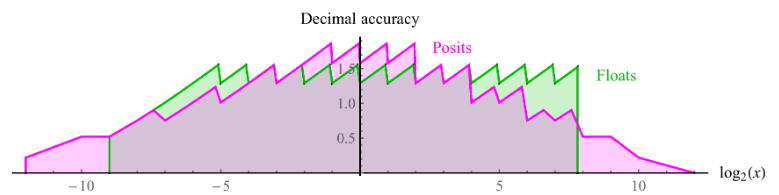
\includegraphics[width=0.9\linewidth]{../Images/decimal_accuracy.png}
	\caption{Image from \cite{posit_arithmetic} showing the decimal accuracy of floating point and posit representatoin as a function of the encoded value}
	\label{fig:deci_accur}
\end{figure}

